\documentclass[a4paper,12pt]{article}

\PassOptionsToPackage{hyphens}{url}\usepackage{hyperref}
\usepackage[parfill]{parskip}
\usepackage[utf8]{inputenc}
\usepackage{listings}
\usepackage{lmodern}
\usepackage{pdflscape}
\usepackage{graphicx}

\newcommand{\mt}{M2CPU}
\newcommand{\mi}{M2 instruction set}
\newcommand{\ma}{M2 architecture}
\newcommand{\inum}{75}

\newcommand{\Ar}{\texttt{A}}
\newcommand{\Gr}{\texttt{G}}
\newcommand{\Hr}{\texttt{H}}
\newcommand{\Xr}{\texttt{X}}
\newcommand{\Yr}{\texttt{Y}}
\newcommand{\Sr}{\texttt{S}}
\newcommand{\SP}{\texttt{SP}}
\newcommand{\PC}{\texttt{PC}}

\title{M2 Architecture And Implementation}
\author{Zakary Nafziger}
\date{15 December 2017}

\begin{document}

\maketitle
\pagenumbering{gobble}
\newpage

\tableofcontents
\pagenumbering{roman}
\newpage

\listoftables
\listoffigures
\newpage

\pagenumbering{arabic}

\section{Introduction}
The \mt{} is a simple subscalar 8-bit processor that implements the \inum{} 
instruction \mi{}. The \mt{} and \mi{} were designed and implemented by the author
as a personal hobby project. The \ma{} is intended to be as simple as possible 
while still being interesting. Some basic information: 
\par

\begin{itemize}
\item 8-bit data and ALU buses
\item 16-bit address bus; 64KB of addressable memory
\item 256B zero-page stack
\item \inum{} instructions
\item implemented in VHDL on a MAX10 based development board
\end{itemize}

This document describes the \mt{}. The \mt{} is only one part of a larger 
project, the M2 computer. As of this writing the other major components of the
M2 computer project are an assembler and VGA video system. The assembler and 
video system are documented separately. 
\par

\subsection{Terminology}
Throughout this document the terms \mt{}, \mi{}, and \ma{} will be used. \mt{} 
refers to the VHDL processor that implements the \mi{}. The \mi{} is the set of
\inum{} instructions that make up the M2 assembly language. The \ma{} refers to the
combination of a processor and instruction set that implement the M2 assembly 
language. The \mt{} is therefore an implementation of the \ma{}, since it 
supports the complete \mi{}. However since the \mt{}'s instructions are 
implemented in microcode it could implement a different architecture. This 
document describes a complete implementation of the \ma{}, namely the \mt{}.
\par

The name 'M2' stands for 'Model 2' The 'Model 1' processor was a 4-bit system 
that was constructed by the Author. The Model 1 was implemented in discrete 
hardware, (about 1200 resistors and transistors). The Model 1 is documented 
here: 
\url{https://hackaday.io/project/665-4-bit-computer-built-from-discrete-transistors}
\par

\newpage
\section{Instruction Set}
The \mt{} implements the \mi{}. The \mi{} is a custom instruction set designed for
this project. The instruction set consists of \inum{} instructions that can be 
broadly grouped into four categories: register manipulation, memory access,
arithmetic and logical, and program control.
\par

\subsection{Register Manipulation Instructions}
The register manipulation instructions allow data to be loaded from one
register to another. The Register manipulation instructions allow completely
orthogonal movement of data between general purpose registers (GPRs), 
restricted data movement between special purpose registers (SPRs) and GPRs, 
and no data movement between two SPRs. Most of the \mt{}'s registers are 8-bits
wide, however the addressing registers may be manipulated 16 bits at a time. 
Each GPR serves a multiple purposes. The primary purpose of the GPRs is to 
provide fast data storage for a program. The secondary purpose(s) of each GPR is
as the target or source of data for a given operation. Each SPR serves a single 
purpose. The Data held in an SPR is always interpreted in a consistent manner. 
The following subsections provide a detailed description of each register's 
function:
\par

\subsubsection{A Register}
The \Ar{} register is an 8-bit GPR. The secondary function of the \Ar{} 
register is as the destination of ALU operations. The result of an ALU 
operation is always stored in the \Ar{} register. The designation '\Ar{}' is 
meant to evoke 'accumulator'.
\par

\subsubsection{G Register}
The \Gr{} register is an 8-bit GPR. The \Gr{} register's secondary function is to hold 
the high byte of an address. Some memory instructions are implicitly addressed 
and since the \mt{} supports a 64KB address space addresses are 16-bits wide.
The low byte of an implicit address is stored in the \Hr{} register. Some 
register manipulation instructions act on the \Gr{} register individually while others
treat the combined \Gr{}\Hr{} register as a single 16-bit unit.
\par

\subsubsection{H Register}
The \Hr{} register is an 8-bit GPR. The \Hr{} register's secondary function is as the 
low byte of an implicit address as described in the previous section.
\par

\subsubsection{X Register}
The \Xr{} register is an 8-bit GPR. The \Xr{} register serves two secondary
purposes. The first is as an ALU operand, and the second is as the point of 
access to the Stack Pointer. Since the Stack Pointer is an SPR it's contents
can only be accessed through a GPR, the \Xr{} register is that GPR.
\par

\subsubsection{Y register}
The \Yr{} register is an 8-bit GPR. The \Yr{} register also serves two 
secondary purposes. The first is as the an ALU operand and the second is as
a point of access to the Status register. In general the \Yr{} register serves
a similar purpose as the \Xr{} register.
\par

\subsubsection{Status Register}
The Status Register (\Sr{} register) is an 8-bit SPR. The low four bits of the
\Sr{} register hold the processor's status flags. The status flags are 
automatically manipulated by the ALU after every arithmetic or logical operation
and may also be manipulated by some control instructions. The status flags are
used by the control instructions to control program flow. The contents of the 
\Sr{} register can be accessed through the \Yr{} register. The status flags are:
\begin{itemize}
\item Zero (\texttt{z}, bit 3). Set when the last ALU operation produced zero as
a result
\item Negative (\texttt{n}, bit 2). Set when the result of the last ALU 
operations was negative (as interpreted in two's complement)
\item Carry (\texttt{c}, bit 1). Set when the result of the last ALU operation
produced a '9th bit', i.e. unsigned addition of two numbers greater than 127.
\item Overflow (\texttt{o}, bit 0). Set when the result of the last ALU 
operation produced an impossible result (when interpreted in two's complement)
\end{itemize}
Status flags are positive logic, i.e. set is '1' and clear is '0'.
\par

\subsubsection{Stack Pointer}
The Stack Pointer (\SP{}) is an 8-bit SPR. The \SP{} holds the address of the 
top of the stack. All stack addresses are mapped onto the zeroth page of memory
and can therefore be represented with a single byte. The \SP{} starts at 
address \texttt{0x0000} and is incremented after each push. This means that the 
stack grows from low addresses to high addresses. The value of the \SP{} can be 
accessed through the \Xr{} register.
\par

\subsubsection{Program Counter}
The Program Counter (\PC{}) is a 16-bit SPR. The \PC{} holds the current memory
address. The \PC{} is incremented after each machine cycle so that the next 
instruction can be fetched. Some instructions may load the \PC{} with a value
other than the next instruction. The \PC{} can be accessed through the combined
\Gr{}\Hr{} register.
\par

\subsection{Memory Manipulation Instructions}
Memory manipulation instructions are instructions that move data from memory to a 
register or from a register to memory. No other category of instruction 
manipulates values in memory. There are three types of memory manipulation 
instruction: direct access, literal to register, and stack operations.
\par

\subsubsection{Direct Access}
Direct Access instructions move a single byte from memory to a given GPR or 
from a given GPR to memory. The address of the byte to manipulate is held in 
the combined \Gr{}\Hr{} register. From a machine language perspective direct 
access instructions look like register manipulation instructions with the added
caveat that the value of the '\texttt{M}' register is dependant on the address
held in the \Gr{}\Hr{} register. In general direct access instructions take 
about twice as long as register manipulation instructions.
\par

\subsubsection{Literal to Register}
Literal to register instructions load a single byte literal in to a given GPR.
Literal to register instructions are similar to direct access instructions,
except that no address is required. The byte to be loaded is stored in the
address immediately following the address storing the instruction code. This
means that these instructions take two addresses when assembled.
\par

\subsubsection{Stack Operations}
Stack operations place a byte on the stack (push) or remove a byte from the
stack (pop) and adjust the \SP{} as necessary. Bytes are pushed from or popped
to GPRs. The stack is stored in the first page of memory; addresses 
\texttt{0x0000} to \texttt{0x00FF}. The \SP{} wraps without warning at the edges
of the stack. This means that stack safety is the sole responsibility of the 
programmer. The \mt{} will happily increment the \SP{} from \texttt{0xFF} to
\texttt{0x00} if a byte is pushed to an already full stack without any type of
warning. This unsafe behaviour was implemented to keep stack instruction 
complexity to a minimum. As it stands stack operations are the most complex and
slow instructions in the \mi{}.
\par

\subsection{Arithmetic and Logical Instructions}
Arithmetic and logical instructions preform an artithmetic or logical function
on the \Xr{} and \Yr{} registers, store the result in the \Ar{} register and 
update the flags in the \Sr{} register. The \mt{}'s ALU can calculate 8 
different functions (detailed in section 2.6). Six of these functions require
two inputs (\Xr{} and \Yr{}), and two functions require only one input, (\Xr{}).
\par

\subsection{Program Control Instructions}
Program control instrcutions control the flow of the program. There are four
types of program control instructions: no-operation, unconditional jump,
conditional branch, and status flag manipulation.
\par

As the name suggests the no-operation does nothing. The no-operation is not 
quite a program control instruction, it is more accurately 'the lack of an 
instruction'. The behaviour of the no-operation is well defined so that if a 
program attempts to execute unitialized memory the processor will behave in a 
predictable (and safe) manner. A no-operation takes an entire machine cycle and
one microstate to execute. More information about machine cycles and 
microstates is found in sections 3.3 and 4 respectively.
\par

\subsubsection{Unconditional Jump}
An unconditional jump sets the address of the next instruction to be executed
as the address held in the \Gr{}\Hr{} register. Since the \PC{} is incremented
at the end of every machine cycle  the jump instruction must decrement the \PC{}
after setting it to the value of the \Gr{}\Hr{} register so that the next 
instruction executed is the one held at the address \Gr{}\Hr{}.
\par

\subsubsection{Conditional Branch}
Conditional branch instructions change which instruction is executed next based 
on the value of a status flag. In general conditional branch instructions allow
the next instruction to be executed if some condition is not met. If the 
condition is met the next instruction is skipped and the instruction following 
it is executed next. This means that the two branches differ by exactly one 
instruction. The condition evaluated is the state of one of the status flags
(section 2.1.6). Since there are four status flags, and each can have two 
values (set or clear) there are eight conditional branch instructions, i.e.
branch if flag set, and branch if flag clear. This branching mechanism is
somewhat austere, however it serves to reduce the overall complexity of the
\mt{}.
\par

Some useful assembly language idioms are the 'escape jump' and 'if-else'. Since
two branches may only differ by one instruction it is often useful to make that 
one instruction an unconditional jump. For example:
\lstset{
	basicstyle=\small\ttfamily
}
\begin{lstlisting}
	LDG 0x0A # load the high byte of 
	         # the escape address 0x0AA0
	LDH 0xA0 # load the low byte of 0x0AA0
	BZC # branch if zero is clear
	JMP # executed if zero is set
	LDX A # executed if zero is clear
	.
	.
	.
	# address 0x0AA0
	LDY A # this code only runs if the 
	      # zero flag was set before the branch.
\end{lstlisting}
An 'if-else' statement can be implemented as follows:
\begin{lstlisting}
	LDX 0x10 # put some data in the X 
	         # and Y registers
	LDY 0x01
	BZS
	LDM X # this instruction is executed
	      # if the zero flag is clear
	BZC
	LDM Y # this instruction is executed
	      # if  the zero flag is set
	... 
	# memory is loaded with X if zero is
	# clear, else memory is loaded with Y
\end{lstlisting}
\par

\subsubsection{Status Flag Manipulation}
Status flag manipulation instructions allow the programmer to set the value of
any of the four status flags. There are 8 status flag manipulation instructions
since each flag can be set ('1') or cleared ('0'). The status flag manipulation
instructions are the only way to move data into the \Sr{} register. The 
contents of the \Sr{} register may be dumped into the \Yr{} register. This 
allows status flags to be stored, or inspected by the program.
\par

\newpage
\section{\mt{} Architecture}
This section outlines the modular architecture of the \mt{}. The implementation
of this architecture is described in section 5. The \mt{} is designed (and 
implemented) as a series of modules that communicate over three major busses. 
The way that these modules interact with each other to carry out instructions is
described in the next section (section 4). In general This section describes the 
processor's 'hardware', whereas section 4 describes how this hardware can be 
made to implement an instruction set.
\par

\subsection{Block Diagram}
The architecture of the \mt{} is well described by a block diagram. Figure 1
shows all of the major components of the processor and is organized very 
similarly to the actual VHDL implementation of the \mt{} (section 5).
\par

\newpage
\thispagestyle{empty}
\begin{landscape}
	\begin{figure}
	\makebox[\linewidth]{
		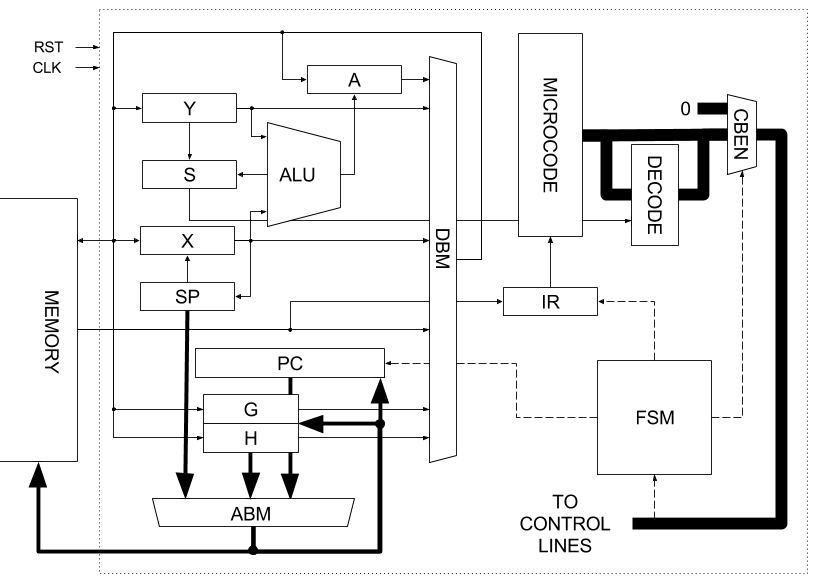
\includegraphics[
			width=18cm,
			height=18cm,
			keepaspectratio
		]{M2CPU_architecture_diagram.png}
	}
	\caption{Simplified \mt{} Block Diagram}
	\end{figure}
\end{landscape}

\newpage
\subsection{Bus Architecture}

\newpage
\section{Control Logic}
\subsection{Machine Cycle}
\subsection{Microcode}

\newpage
\section{VHDL Implementation}

\newpage

\section{Detailed Instruction Descriptions}
This section provides a detailed description of each instruction in the \mi{}.
Some instructions are very similar, as such they have been grouped for 
convenience. A discription of each instruction's microstates is also included.
This section is included primarily as technical reference. High level 
descriptions of the instruction set and the microcode implementation are provided
in sections 2 and 4 respectively. Table 1 (section 6.14) provides a handy 
programming reference.
\par
\subsection{Load GPR}
\subsection{Load SPR}
\subsection{Load Memory From GPR}
\subsection{Load GPR From Memory}
\subsection{Load GPR With Literal}
\subsection{Push GPR}
\subsection{Pop GPR}
\subsection{ALU Operations}
\subsection{Set Status Flag}
\subsection{Clear Status Flag}
\subsection{Conditional Branch}
\subsection{No-operation}
\subsection{Jump}
\subsection{Instruction Table}
Table 1 shows each instruction and its corresponding hexadecimal code. Each
instruction is a single byte long, some instructions take a single byte-literal 
argument represented with a '\texttt{\#}'. The hexadecimal code (microaddress) 
for a a given instruction is found by adding the high nybble (row) and low 
nybble (column). Detailed descriptions each instruction are provided in 
sections 6.1 to 6.13.
\par

\newpage
\thispagestyle{empty}
\begin{landscape}
\begin{table}
	\makebox[\linewidth]{
		\texttt{
		\begin{tabular}{ c c|c|c|c|c|c|c|c|c|c|c|c|c|c|c|c|c|}
			\cline{3-18}
			&&\multicolumn{16}{|c|}{LOW NYBBLE} \\ 
			\cline{3-18}
			&&0x00&0x01&0x02&0x03&0x04&0x05&0x06&0x07&0x08&0x09&0x0A&0x0B&0x0C&0x0D&0x0E&0x0F \\ \hline
			\multicolumn{1}{|c|}{}&0x00&NOP&LDA G&&LDA H&&LDA X&&LDA Y&&LDSP X&&&ADD&&BZS& \\ \cline{2-18}
			\multicolumn{1}{|c|}{}&0x10&&LDG A&&LDG H&&LDG X&&LDG Y&&LDX SP&&&SUB&&BZC& \\ \cline{2-18}
			\multicolumn{1}{|c|}{H}&0x20&&LDH A&&LDH G&&LDH X&&LDH Y&&LDY S&&&AND&&BNS& \\ \cline{2-18}
			\multicolumn{1}{|c|}{I}&0x30&&LDX A&&LDX G&&LDX H&&LDX Y&&LDGH PC&&&NND&&BNC& \\ \cline{2-18}
			\multicolumn{1}{|c|}{G}&0x40&&LDY A&&LDY G&&LDY H&&LDY X&&JMP&&&ORR&&BCS& \\ \cline{2-18}
			\multicolumn{1}{|c|}{H}&0x50&&&&&&&&&&&&&XOR&&BCC& \\ \cline{2-18}
			\multicolumn{1}{|c|}{}&0x60&LDM A&&&LDA M&&&&LDA \#&&&&&STL&&BOS& \\ \cline{2-18}
			\multicolumn{1}{|c|}{N}&0x70&LDM G&&&LDG M&&&&LDG \#&&&&&STR&&BOC& \\ \cline{2-18}
			\multicolumn{1}{|c|}{Y}&0x80&LDM H&&&LDH M&&&&LDH \#&&&&&&&SZF& \\ \cline{2-18}
			\multicolumn{1}{|c|}{B}&0x90&LDM X&&&LDX M&&&&LDX \#&&&&&&&CZF& \\ \cline{2-18}
			\multicolumn{1}{|c|}{B}&0xA0&LDM Y&&&LDY M&&&&LDY \#&&&&&&&SNF& \\ \cline{2-18}
			\multicolumn{1}{|c|}{L}&0xB0&PHA&&&&&PPA&&&&&&&&&CNF& \\ \cline{2-18}
			\multicolumn{1}{|c|}{E}&0xC0&PHG&&&&&PPG&&&&&&&&&SCF& \\ \cline{2-18}
			\multicolumn{1}{|c|}{}&0xD0&PHH&&&&&PPH&&&&&&&&&CCF& \\ \cline{2-18}
			\multicolumn{1}{|c|}{}&0xE0&PHX&&&&&PPX&&&&&&&&&SOF& \\ \cline{2-18}
			\multicolumn{1}{|c|}{}&0xF0&PHY&&&&&PPY&&&&&&&&&COF& \\ \hline
		\end{tabular}
		}
	}
	\caption{The M2 Instruction Set}
\end{table}
\end{landscape}

\newpage
\section{Conclusion}

\end{document}
